\section{Baricentro de Wasserstein Bayesiano}\label{sec:bwb}  % MARK: - Section Baricentro de Wasserstein Bayesiano


Si es que se tiene un conjunto de modelos finito $\Models \subseteq \ProbSpace[\cX] $ con $| \Models | = N < + \infty$, por definición, la medida posterior corresponde a una medida discreta. En este caso, se puede calcular el vector de verosimilitudes $L_n = (\cL_n(\mu))_{\mu \in \Models} \in \R^N$ y normalizarlo, para obtener el vector de probabilidades de la posterior. En este enfoque, se muestrea un índice $i$ con probabilidad proporcional a $L_n$ y devuelve el modelo $\mu_i$.

Esta estrategia resulta muy conveniente cuando los modelos de $\Manifold$ poseen densidad en $\R^d$ y los datos $\Data$ se encuentran en los soportes de $\mu\in \Manifold$. Sin embargo, para el contexto de esta tesis, en la que se desea calcular el baricentro de un conjunto de imágenes, es muy frecuente que la verosimilitud sea nula. Esto resulta en que el soporte de la medida posterior sea bastante menor al original. Es más, cuando el número de datos $\Data$ aumenta, incluso para números muy pequeños, como $n=20$, el soporte de la posterior se reduce rápidamente. Por estos motivos, se decide tomar otro enfoque, el cual se presenta en la siguiente sección.


\subsection{Construcción de la Posterior Usando una GAN}\label{ssec:construccion-posterior}  % MARK: - Construcción de la Posterior Usando una GAN

Como se explicó en secciones anteriores,\FM{Aquí sería bueno incluir las secciones de lo que se habla esto, sguramente el de la GAN y WGAN}
dada una medida de referencia $\Prob_X$\footnote{Del cuál se tiene acceso a través de una estimación por medio de la medida empírica $\hat\Prob_X = \frac{1}{N}\sum_{i=1}^{N} \delta_{x_i}$, donde $x_i \sim \Prob_X$.}, lo que hacen las redes generativas es aproximarla por medio de un modelo generativo $\Prob_G$. Gracias a esta propiedad, se propone utilizar una GAN como prior para poder calcular la posterior.

Cabe destacar que la idea de utilizar una GAN como prior se encuentra en un trabajo previo \cite{patel2019bayesian}, pero este presenta fallos en su planteamiento. Por lo tanto, en este trabajo de tesis se solucionan y formalizan los errores cometidos en el trabajo anterior.\RED{Hay que revisar este último párrafo.}

Dada una red generadora $G_\theta \colon \cZ \to \ProbSpace[\cX] $ con una medida en el espacio latente $\Prob_Z$, se propone utilizar como prior a la medida
\begin{equation}
    \Pi^G \eqdef \pf{G_\theta} \Prob_Z.
\end{equation}
De esta manera, la posterior tendría la siguiente forma:
\begin{equation}
    \Pi_n(\dd \mu)
    \eqdef \frac{\cL_n(\mu)}{\int_{\ProbSpace[\cX]} \cL_n(\nu) \; \Pi^G(\dd \nu)} \; \Pi^G(\dd \mu)
    = C^{-1} \cL_n(\mu) \; \Pi^G(\dd \mu),
\end{equation}
donde $C \eqdef \int_{\ProbSpace[\cX]} \cL_n(\nu) \; \Pi^G(\dd \nu)$ es una constante de normalización.

Dada una función arbitraria $g$ $\Pi_n$-integrable (como por ejemplo, la función $\mu \mapsto \Wasserstein[p]{\mu}{\nu}^p$), se puede comprobar lo siguiente:
\begin{align}\label{eq:posterior-en-latente-deduccion}
     & \int_{\ProbSpace[\cX]} g(\mu) \; \Pi_n(\dd \mu)                         \\
     & = C^{-1} \int_{\ProbSpace[\cX]} g(\mu) \cL_n(\mu) \; \Pi^G(\dd \mu)     \\
     & = C^{-1} \int_{\cZ} g(G_\theta(z)) \cL_n(G_\theta(z)) \; \Prob_Z(\dd z) \\
     & = \int_{\cZ} g(G_\theta(z)) \; \Pi^Z_n(\dd z),
\end{align}
donde $\Pi^Z_n(\dd z)$ es la \textit{medida posterior en el espacio latente}, y se define por
\begin{equation}
    \Pi^Z_n(\dd z) \eqdef C^{-1} \cL_n(G_\theta(z)) \; \Prob_Z(\dd z).
\end{equation}

Por la Definición~\ref{def:operador-push-forward} del operador push-forward, se concluye la siguiente propiedad de la medida posterior:
\begin{equation}\label{eq:posterior-en-latente}
    \Pi_n = \pf{G_\theta} \Pi^Z_n.
\end{equation}
La forma de interpretar la ecuación anterior, es que para obtener un muestreo de la posterior $\mu\sim\Pi_n$ basta con hacer un muestreo $z\sim\Pi^Z_n$ y después aplicar la red generadora $G_\theta$ sobre $z$.

Esto resulta beneficioso, pues delega la tarea de realizar un muestreo a partir de la posterior al espacio latente $\cZ$ (el cuál, en la práctica, es $\R^{d_z}$), la cual es mucho más fácil de simular. Por ejemplo, una manera de obtener muestreos a partir de $\Pi^Z_n$, es por medio del método de Markov Chain Monte Carlo (MCMC) \cite{andrieu2003introduction,brooks2011handbook,goodman2010ensemble}.

\subsubsection{Simulación de la Posterior}\label{sssec:sim-posterior}  % MARK: - Simulación de la Posterior

Sea un modelo $\tilde\mu\in \Manifold$ fijo. Si $\Data \eqdef \left\{ x_i \right\}_{i=1}^n \sim$ son $n$ datos a partir de $\tilde\mu$, se desea comprobar si las muestras de la posterior $\Pi_n$ son parecidos al modelo original $\tilde\mu$. Se espera que a medida que $n$ aumente, las muestras de la posterior se parezcan más al modelo original.

Para ello, se seleccionará un modelo $\tilde\mu\in \Manifold$ que corresponde a una imgaen y se muestrearán $n$ datos $\Data = \left\{ x_i \right\}_{i=1}^n$ a partir de $\tilde\mu$ para $n\in\left\{ 5, 20, 50, 100 \right\}$.
En la Figura~\ref{fig:image-sampler-i-37} se muestra el modelo $\tilde\mu$ seleccionado.
\begin{figure}[H]
    \centering
    
\includegraphics[width=0.33\textwidth]{img/mcmc/image-sampler-i-37.pdf}
    \caption{Imagen $\tilde\mu\in \Manifold$ de donde se muestrearán los datos.}
    \label{fig:image-sampler-i-37}
\end{figure}

A partir de la Ecuación~\ref{eq:posterior-en-latente}, se puede determinar la función de densidad de la medida $\Pi^Z_n$:
\begin{align}
    \rho_{\Pi^Z_n}(z)
     & = \frac{1}{C} \cL_n(G_\theta(z)) \frac{1}{\sqrt{2\pi}^{d_z}} \exp\left( -\frac{1}{2} \| z \|_2^2 \right)         \\
     & \propto \cL_n(G_\theta(z)) \exp\left( -\frac{1}{2} \| z \|_2^2 \right). \label{eq:posterior-en-latente-densidad}
\end{align}
donde se asume que la distribución del espacio latente $\Prob_Z$ es una distribución normal estándar en $\R^{d_z}$.
Gracias a que se tiene acceso a la función de densidad de $\Pi^Z_n$, se puede utilizar la técnica de MCMC para simular muestras de la posterior $\Pi_n$. En particular, se utilizará el Muestreador No-U-Turn (NUTS por sus siglas en inglés) \cite{hoffman2014no} utilizando la implementación de \textit{hamiltorch} \cite{cobb2019introducing}.

Para la función potencial, se tomará el negativo del logaritmo de la Ecuación~\ref{eq:posterior-en-latente-densidad}, salvo las constantes de normalización:
\begin{align}
    U(z)
     & = -\log\left( \cL_n(G_\theta(z)) \right) - \log\left(
    \exp\left( -\frac{1}{2} \| z \|_2^2 \right)
    \right)                                                  \\
     & = -\sum_{i=1}^{n} \log\left( \nu_z(x_i) \right)
    + \frac{1}{2} \| z \|_2^2,
\end{align}
donde $\nu_z = G_\theta(z)$, mientras que para el primer término se utiliza el hecho de que $\cL_n(\nu_z) = \prod_{i=1}^{n} \nu_z(x_i)$. Para los expermientos, se realizan muestreos para $n \in \left\{ 5, 20, 50, 100 \right\}$, en donde cada experimento se ejecutaron $8$ cadenas en paralelo, donde cada una realiza $150.000$ pasos del MCMC con un \textit{burn-in} de $2.000$ pasos. Los resultados de los experimentos se pueden observar en las Figuras~\ref{fig:mcmc-n-005}, \ref{fig:mcmc-n-020}, \ref{fig:mcmc-n-050} y \ref{fig:mcmc-n-100} respectivamente. En cada una de las figuras, se adjunta una estimación del tiempo de autocorrelación promedio, calculado con una adaptación de la función \texttt{autocorr} de la librería \textit{emcee} \cite{foreman2013emcee}.

% Caso n=5
\begin{figure}[H]
    \centering
    \begin{subfigure}[t]{0.35\textwidth}
        \centering
        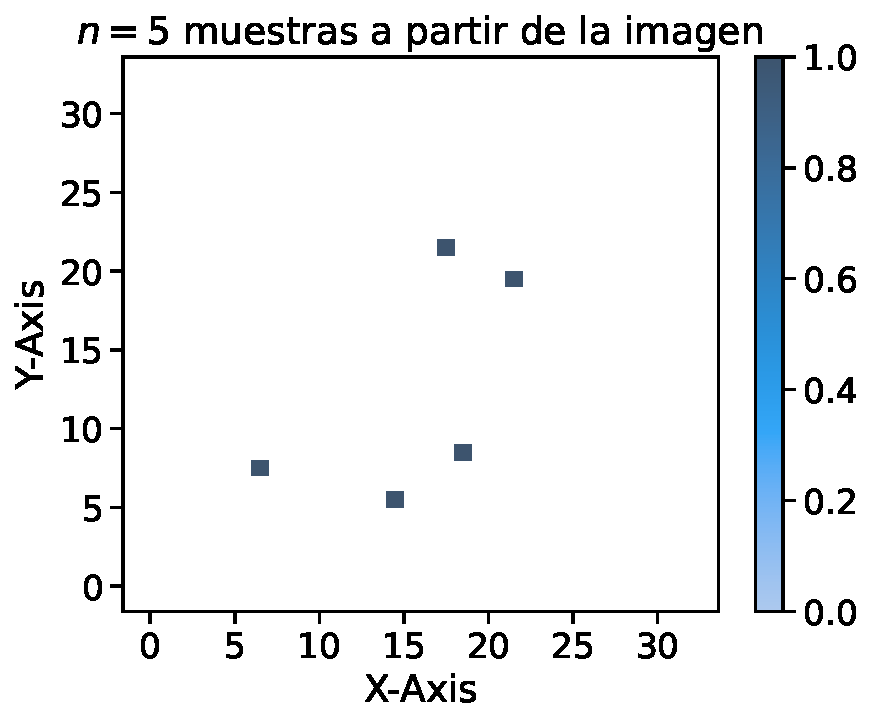
\includegraphics[width=\textwidth]{img/mcmc/samples-hist-n-005.pdf}
        \caption{Histograma de los datos.}
        \label{fig:samples-hist-n-005}
    \end{subfigure}
    \hfill
    \begin{subfigure}[t]{0.59\textwidth}
        \centering
        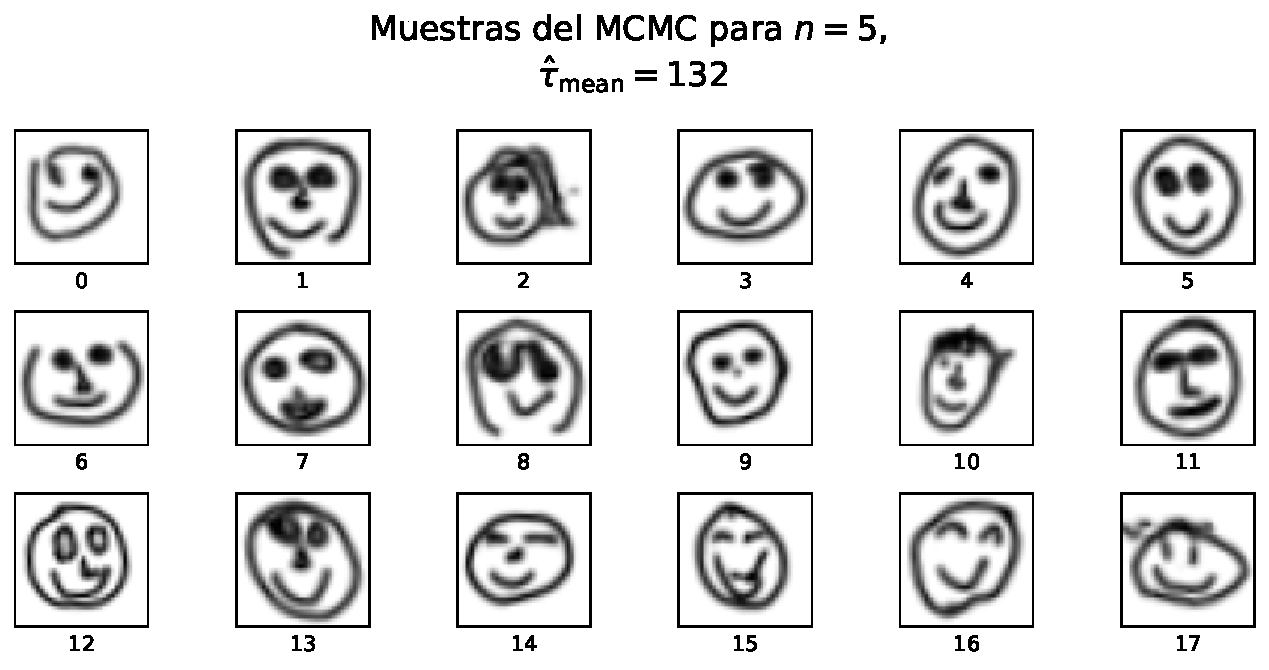
\includegraphics[width=\textwidth]{img/mcmc/mcmc-n-005-NUTSPosteriorSampler.pdf}
        \caption{Muestras de la posterior.}
        \label{fig:mcmc-n-005-NUTSPosteriorSampler}
    \end{subfigure}
    \caption{Muestras de la posterior $\Pi^Z_n$ a partir de $n=5$ datos.}
    \label{fig:mcmc-n-005}
\end{figure}

% Caso n=20
\begin{figure}[H]
    \centering
    \begin{subfigure}[t]{0.35\textwidth}
        \centering
        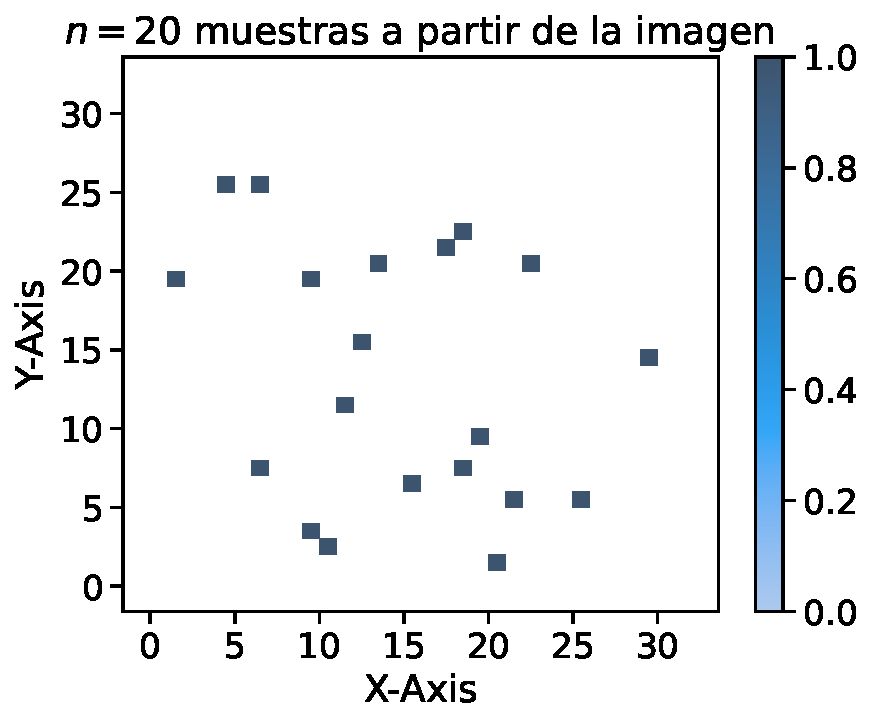
\includegraphics[width=\textwidth]{img/mcmc/samples-hist-n-020.pdf}
        \caption{Histograma de los datos.}
        \label{fig:samples-hist-n-020}
    \end{subfigure}
    \hfill
    \begin{subfigure}[t]{0.59\textwidth}
        \centering
        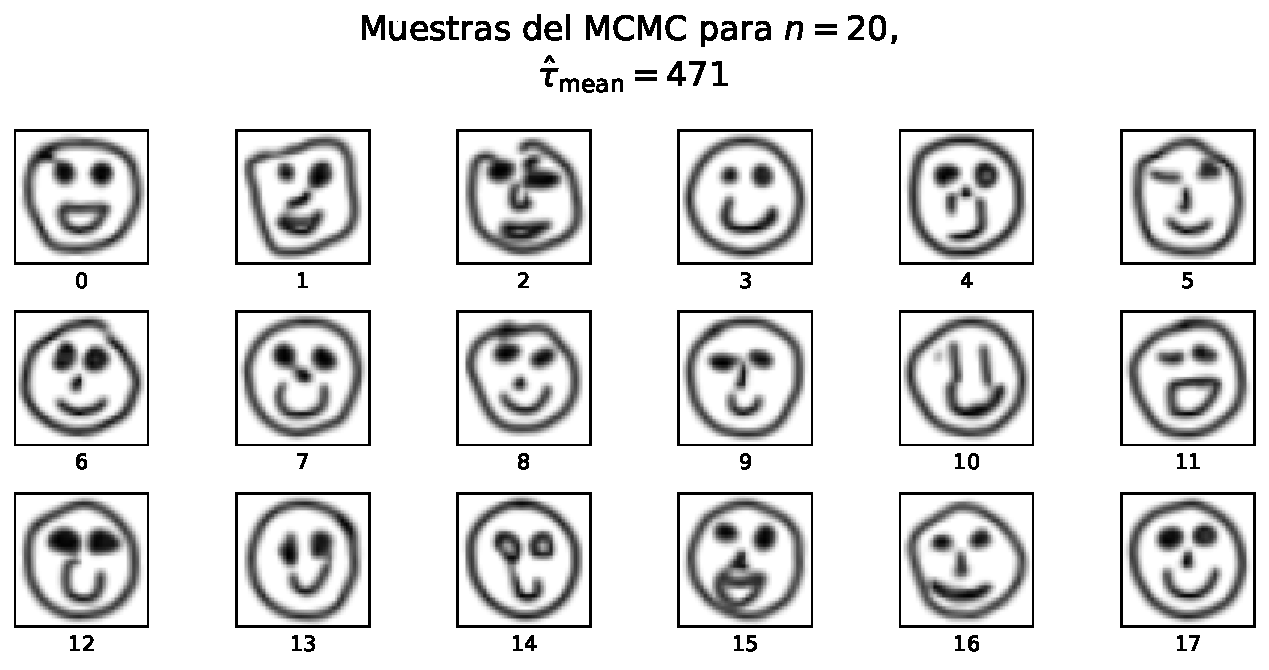
\includegraphics[width=\textwidth]{img/mcmc/mcmc-n-020-NUTSPosteriorSampler.pdf}
        \caption{Muestras de la posterior.}
        \label{fig:mcmc-n-020-NUTSPosteriorSampler}
    \end{subfigure}
    \caption{Muestras de la posterior $\Pi^Z_n$ a partir de $n=20$ datos.}
    \label{fig:mcmc-n-020}
\end{figure}

% Caso n=50
\begin{figure}[H]
    \centering
    \begin{subfigure}[t]{0.35\textwidth}
        \centering
        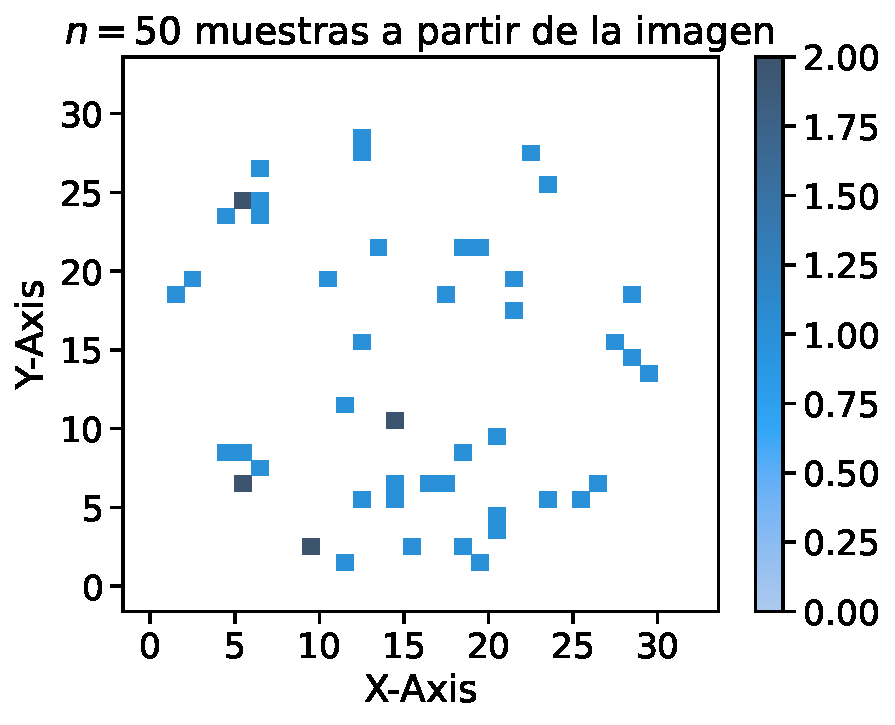
\includegraphics[width=\textwidth]{img/mcmc/samples-hist-n-050.pdf}
        \caption{Histograma de los datos.}
        \label{fig:samples-hist-n-050}
    \end{subfigure}
    \hfill
    \begin{subfigure}[t]{0.59\textwidth}
        \centering
        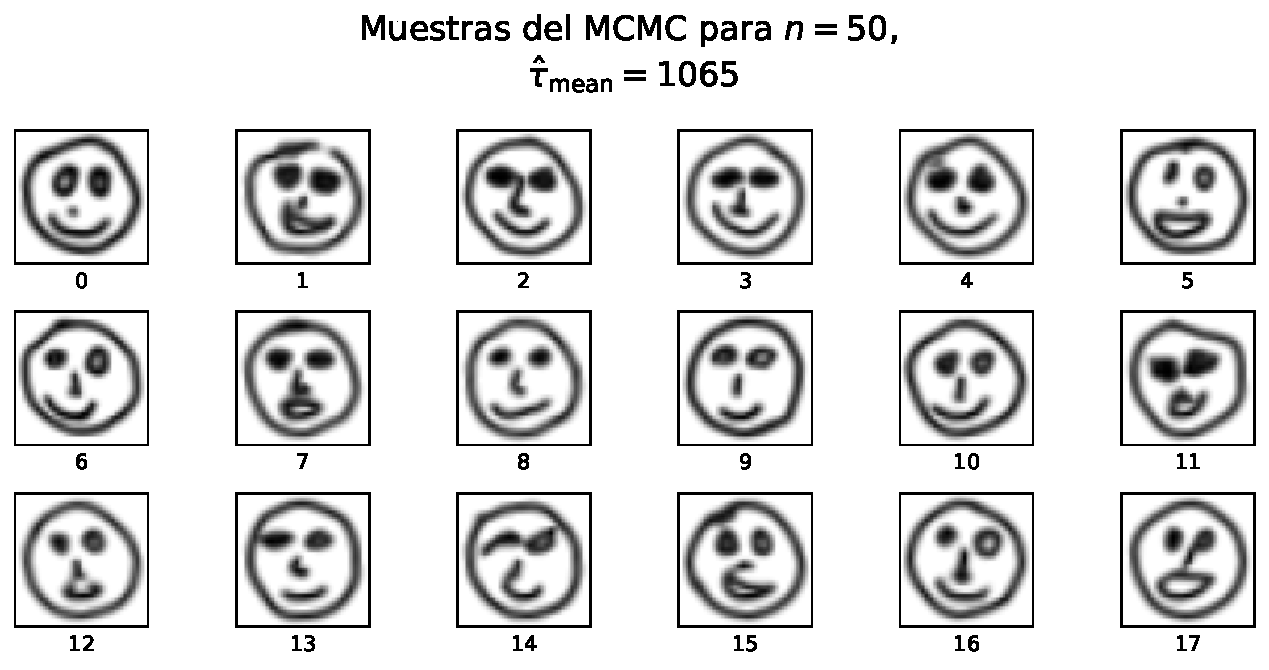
\includegraphics[width=\textwidth]{img/mcmc/mcmc-n-050-NUTSPosteriorSampler.pdf}
        \caption{Muestras de la posterior.}
        \label{fig:mcmc-n-050-NUTSPosteriorSampler}
    \end{subfigure}
    \caption{Muestras de la posterior $\Pi^Z_n$ a partir de $n=50$ datos.}
    \label{fig:mcmc-n-050}
\end{figure}

% Caso n=100
\begin{figure}[H]
    \centering
    \begin{subfigure}[t]{0.35\textwidth}
        \centering
        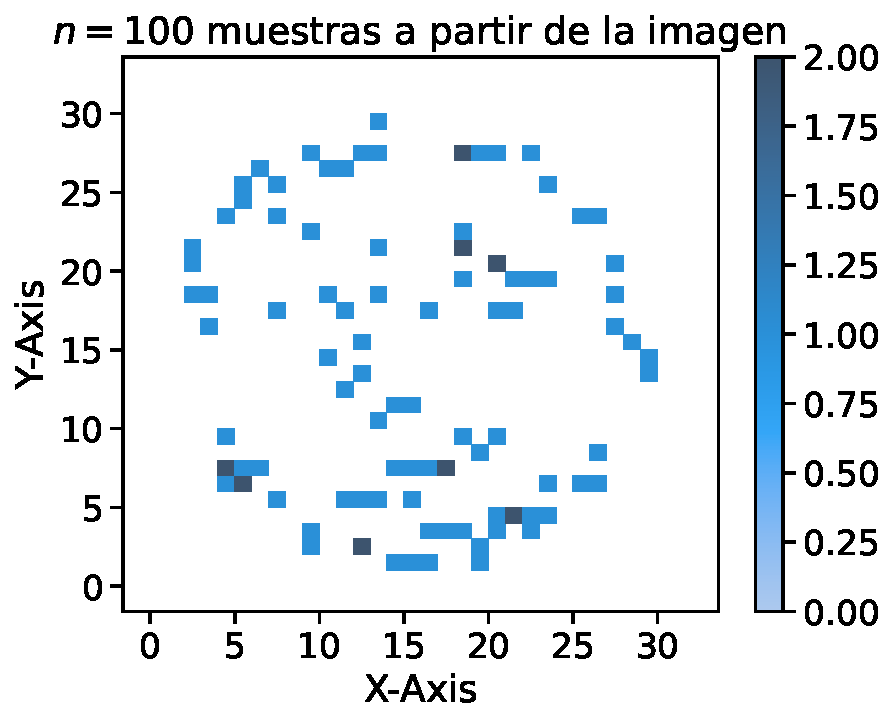
\includegraphics[width=\textwidth]{img/mcmc/samples-hist-n-100.pdf}
        \caption{Histograma de los datos.}
        \label{fig:samples-hist-n-100}
    \end{subfigure}
    \hfill
    \begin{subfigure}[t]{0.59\textwidth}
        \centering
        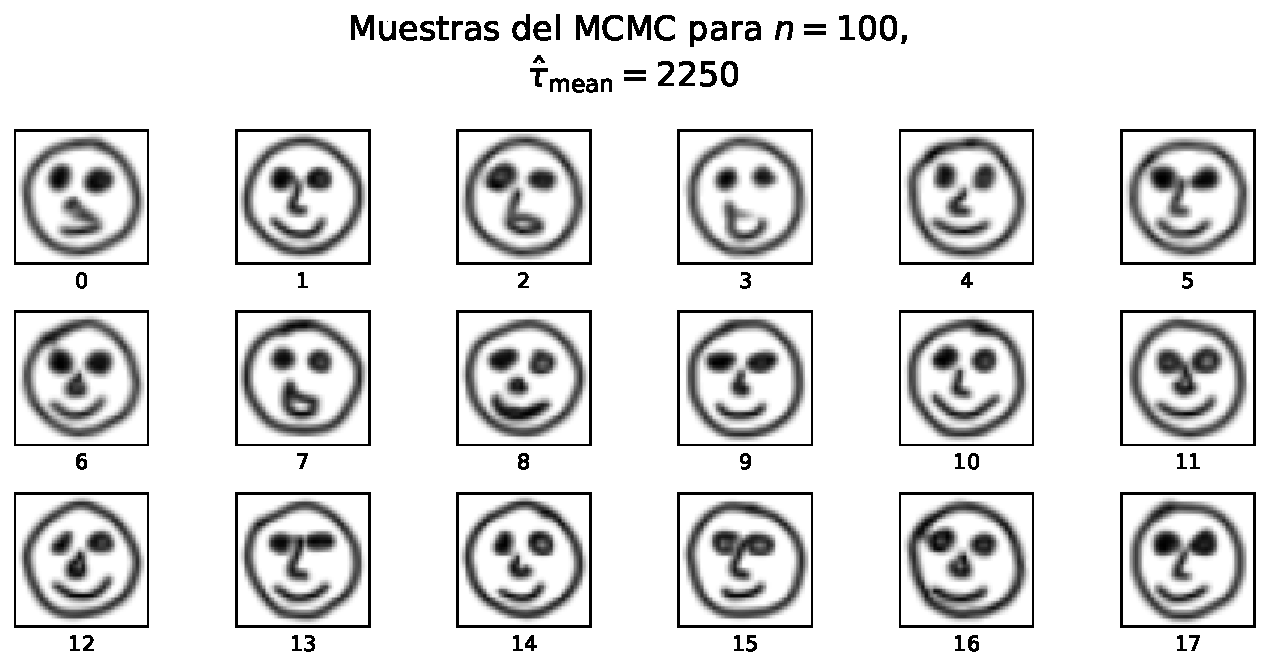
\includegraphics[width=\textwidth]{img/mcmc/mcmc-n-100-NUTSPosteriorSampler.pdf}
        \caption{Muestras de la posterior.}
        \label{fig:mcmc-n-100-NUTSPosteriorSampler}
    \end{subfigure}
    \caption{Muestras de la posterior $\Pi^Z_n$ a partir de $n=100$ datos.}
    \label{fig:mcmc-n-100}
\end{figure}

A partir de las Figuras~\ref{fig:mcmc-n-005}, \ref{fig:mcmc-n-020}, \ref{fig:mcmc-n-050} y \ref{fig:mcmc-n-100}, se puede observar que a medida que se aumenta el número de datos $n$, las muestras de la posterior $\Pi^Z_n$ se parecen más al modelo original $\tilde\mu$. Esto es lo esperable en un enfoque Bayesiano.

\subsection{Cálculo del Baricentro de Wasserstein Bayesiano}\label{ssec:calc-bwb}  % MARK: - Cálculo del Baricentro de Wasserstein Bayesiano

\RED[inline]{Revisar esta sección}
Ahora que se conoce que se pueden simular muestras de la posterior $\Pi_n$ a partir de una red generativa, se puede calcular el baricentro de Wasserstein Bayesiano. Para ello, se utilizará el algoritmo de SGDW presentada en la Sección~\ref{sec:sgdw} con distintos valores de $n$ para observar cómo se comporta el baricentro a medida que se aumenta el número de datos.

En la sección anterior se observa que con $n = 50$ ya hay muestras muy similares a la imagen original. Por este motivo, se realizarán experimentos con $n \in \left\{ 5, 10, 25, 50 \right\}$. Para el MCMC se utilizará $16$ cadenas diferentes de un largo de $25\,000$ cada una, quemando los primeros $2\,500$ pasos.
Y para los parámetros del SGDW se utilizarán los mismos que en la Sección~\ref{sec:sgdw}.\FM{\textbf{Esto también puede cambiar.}}


% \begin{figure}[H]
%     % n = 5
%     \begin{subfigure}[t]{0.49\textwidth}
%         \centering
%         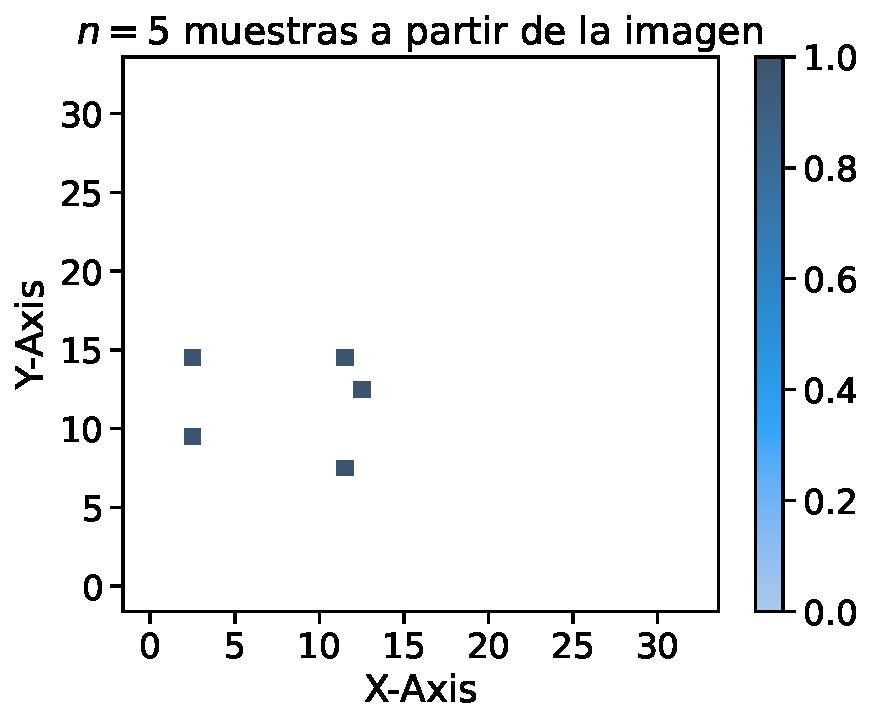
\includegraphics[height=6cm]{img/bwb/samples-hist-n-05.pdf}
%         \caption{Histograma de los datos con $n=5$.}
%         \label{fig:samples-hist-n-05}
%     \end{subfigure}
%     \hfill
%     \begin{subfigure}[t]{0.49\textwidth}
%         \centering
%         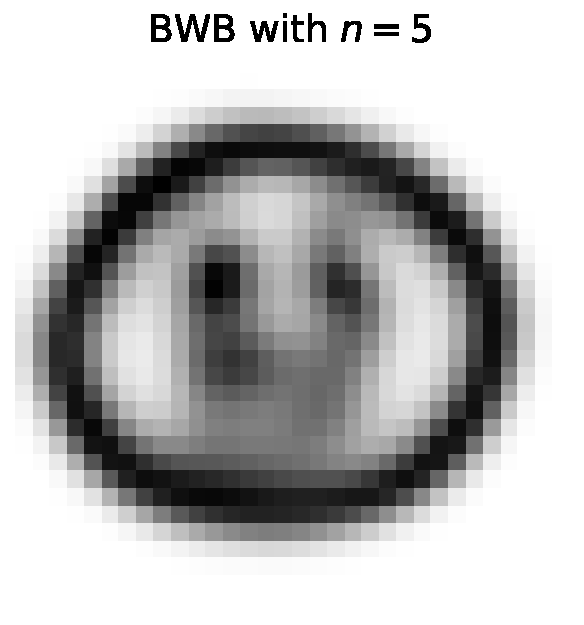
\includegraphics[height=6cm]{img/bwb/BWB-n-data-05.pdf}
%         \caption{Baricentro con $n=5$.}
%         \label{fig:bwb-n-data-05}
%     \end{subfigure}
%     % n = 10
%     \begin{subfigure}[t]{0.49\textwidth}
%         \centering
%         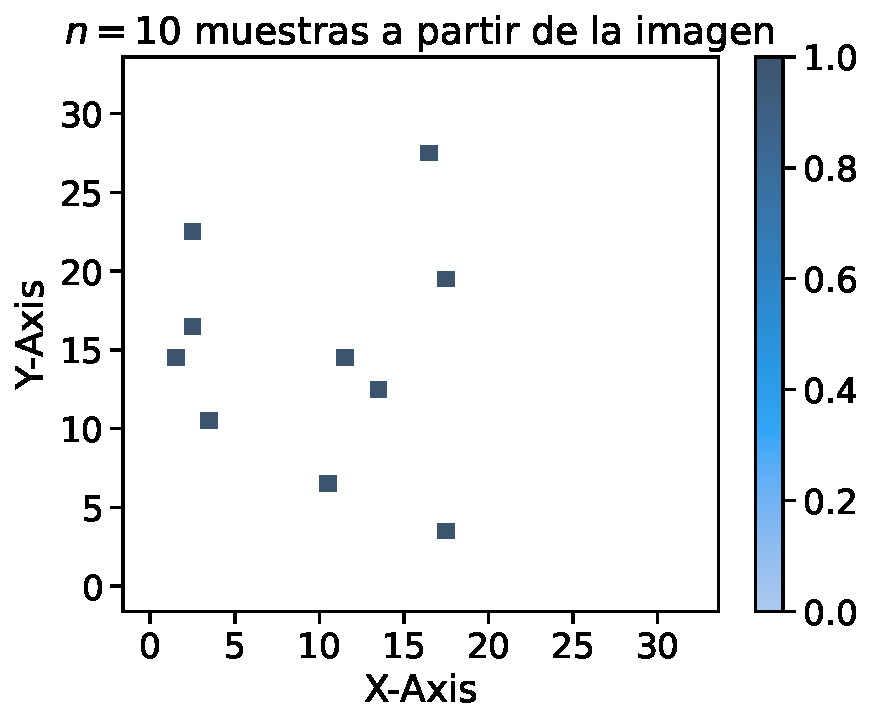
\includegraphics[height=6cm]{img/bwb/samples-hist-n-10.pdf}
%         \caption{Histograma de los datos con $n=10$.}
%         \label{fig:samples-hist-n-10}
%     \end{subfigure}
%     \hfill
%     \begin{subfigure}[t]{0.49\textwidth}
%         \centering
%         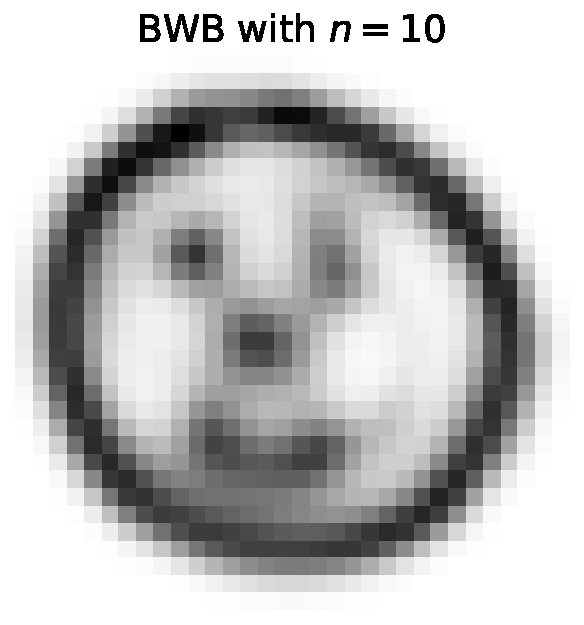
\includegraphics[height=6cm]{img/bwb/BWB-n-data-10.pdf}
%         \caption{Baricentro con $n=10$.}
%         \label{fig:bwb-n-data-10}
%     \end{subfigure}
%     % n = 25
%     \begin{subfigure}[t]{0.49\textwidth}
%         \centering
%         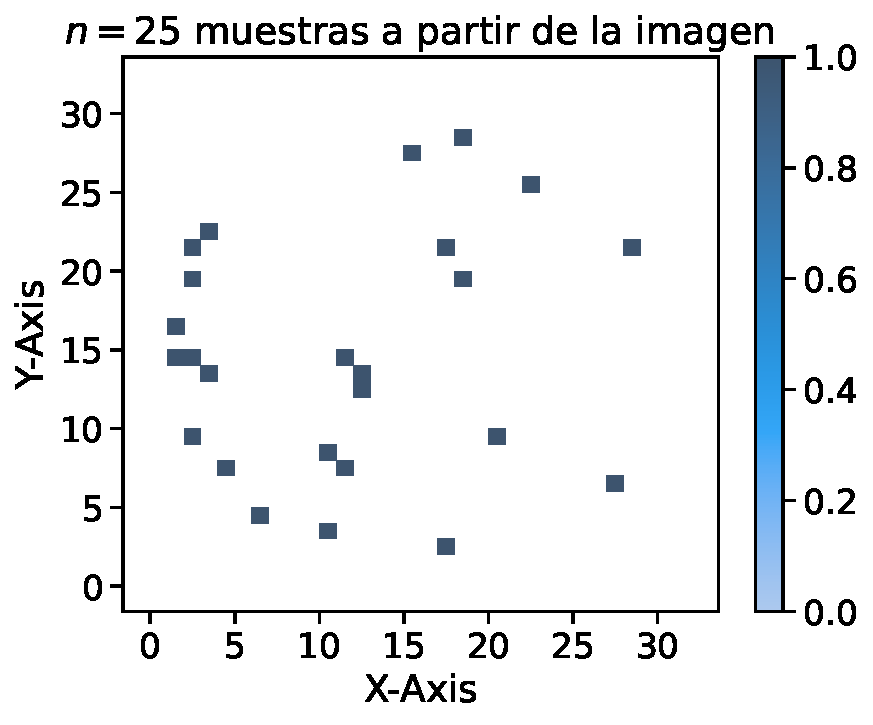
\includegraphics[height=6cm]{img/bwb/samples-hist-n-25.pdf}
%         \caption{Histograma de los datos con $n=25$.}
%         \label{fig:samples-hist-n-25}
%     \end{subfigure}
%     \hfill
%     \begin{subfigure}[t]{0.49\textwidth}
%         \centering
%         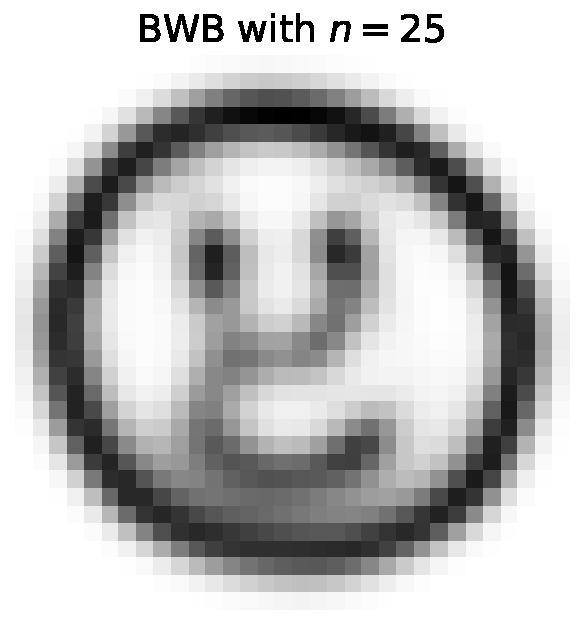
\includegraphics[height=6cm]{img/bwb/BWB-n-data-25.pdf}
%         \caption{Baricentro con $n=25$.}
%         \label{fig:bwb-n-data-25}
%     \end{subfigure}
%     % n = 50
%     \begin{subfigure}[t]{0.49\textwidth}
%         \centering
%         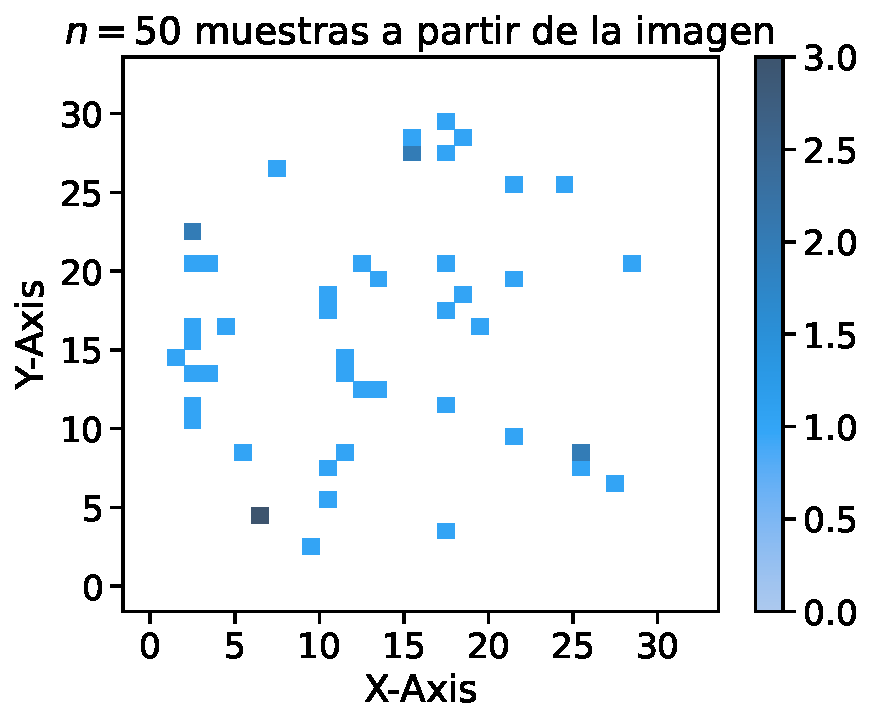
\includegraphics[height=6cm]{img/bwb/samples-hist-n-50.pdf}
%         \caption{Histograma de los datos con $n=50$.}
%         \label{fig:samples-hist-n-50}
%     \end{subfigure}
%     \hfill
%     \begin{subfigure}[t]{0.49\textwidth}
%         \centering
%         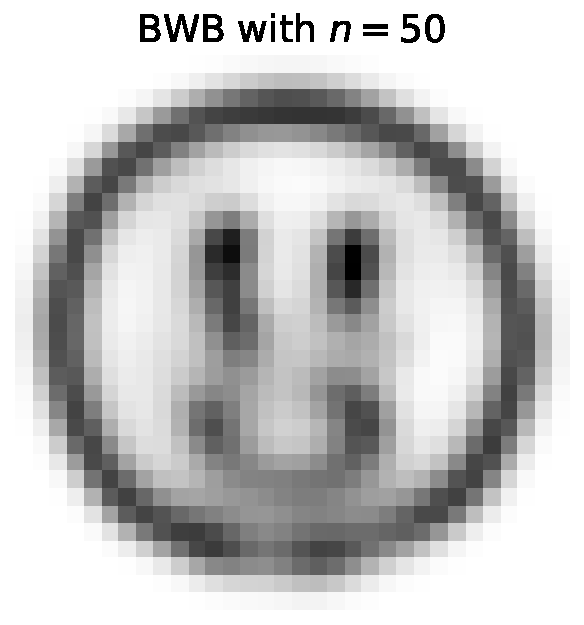
\includegraphics[height=6cm]{img/bwb/BWB-n-data-50.pdf}
%         \caption{Baricentro con $n=50$.}
%         \label{fig:bwb-n-data-50}
%     \end{subfigure}
%     \caption{Resultados de los experimentos para el cálculo del baricentro de Wasserstein Bayesiano.}
%     \label{fig:bwb-experiments}
% \end{figure}

% n = 5
\begin{figure}[H]
    \begin{subfigure}[t]{0.49\textwidth}
        \centering
        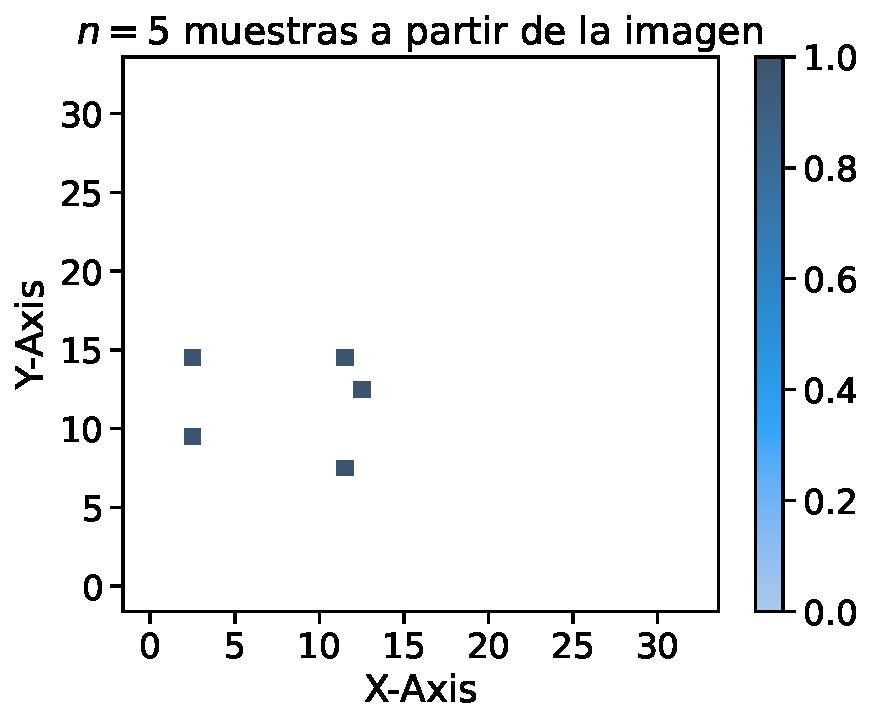
\includegraphics[height=6cm]{img/bwb/samples-hist-n-05.pdf}
        \caption{Histograma de los datos con $n=5$.}
        \label{fig:samples-hist-n-05}
    \end{subfigure}
    \hfill
    \begin{subfigure}[t]{0.49\textwidth}
        \centering
        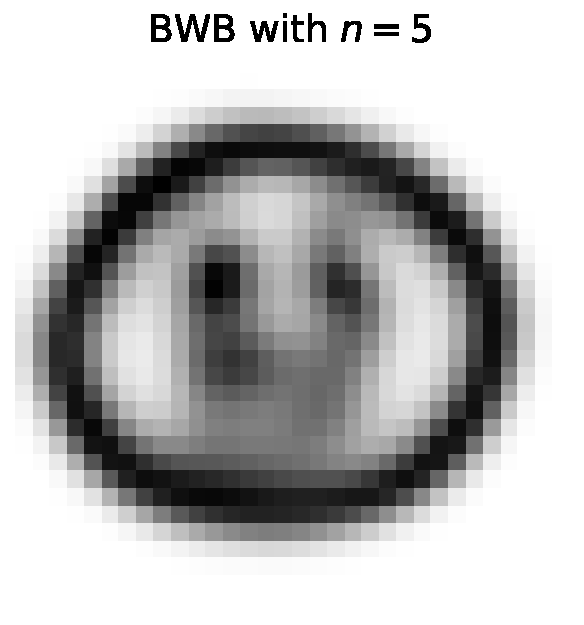
\includegraphics[height=6cm]{img/bwb/BWB-n-data-05.pdf}
        \caption{Baricentro con $n=5$.}
        \label{fig:bwb-n-data-05}
    \end{subfigure}
    \caption{Resultados de los experimentos para el cálculo del BWB con $n=5$.}
    \label{fig:bwb-experiments-n-05}
\end{figure}

% n = 10
\begin{figure}[H]
    \begin{subfigure}[t]{0.49\textwidth}
        \centering
        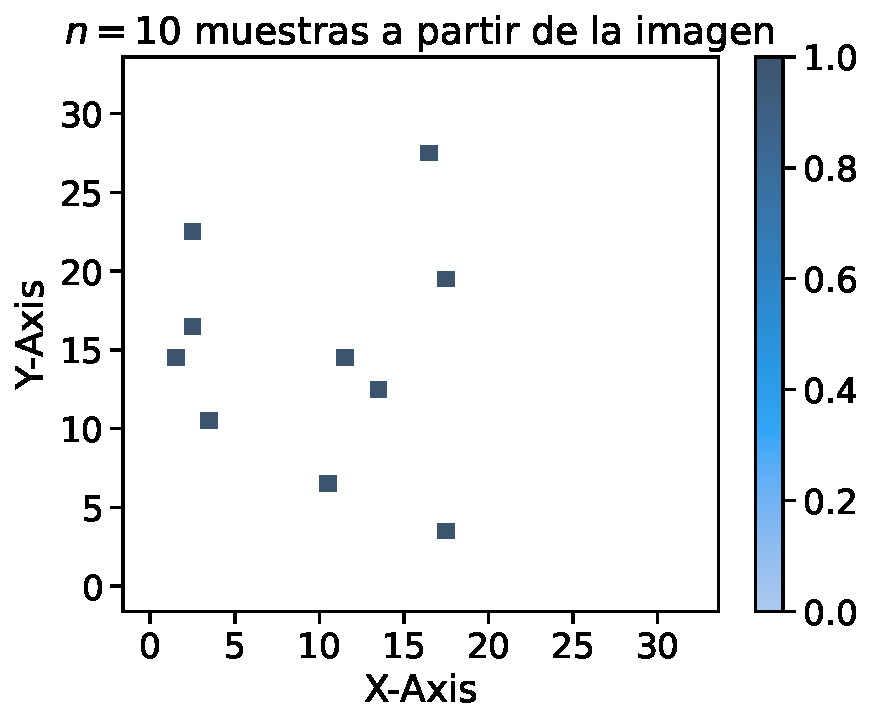
\includegraphics[height=6cm]{img/bwb/samples-hist-n-10.pdf}
        \caption{Histograma de los datos con $n=10$.}
        \label{fig:samples-hist-n-10}
    \end{subfigure}
    \hfill
    \begin{subfigure}[t]{0.49\textwidth}
        \centering
        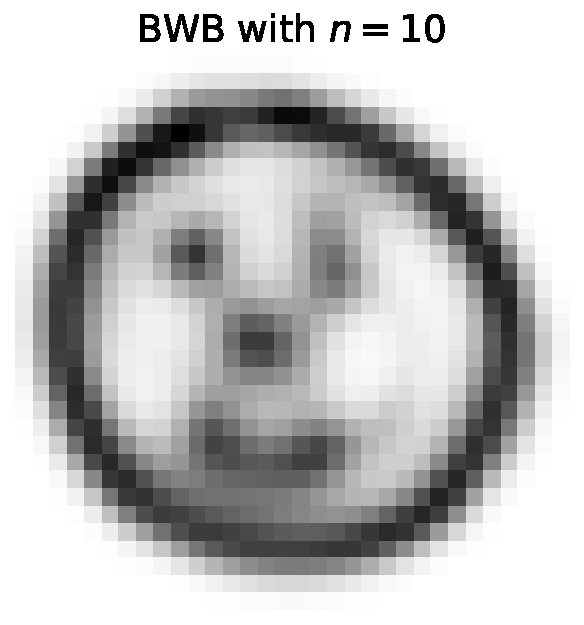
\includegraphics[height=6cm]{img/bwb/BWB-n-data-10.pdf}
        \caption{Baricentro con $n=10$.}
        \label{fig:bwb-n-data-10}
    \end{subfigure}
    \caption{Resultados de los experimentos para el cálculo del BWB con $n=10$.}
    \label{fig:bwb-experiments-n-10}
\end{figure}

% n = 25
\begin{figure}[H]
    \begin{subfigure}[t]{0.49\textwidth}
        \centering
        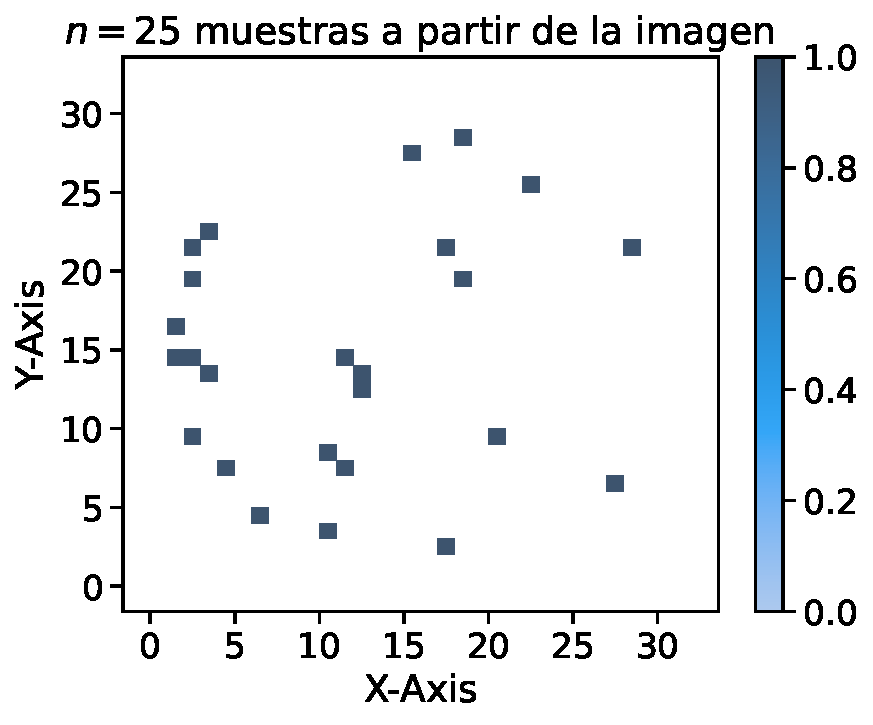
\includegraphics[height=6cm]{img/bwb/samples-hist-n-25.pdf}
        \caption{Histograma de los datos con $n=25$.}
        \label{fig:samples-hist-n-25}
    \end{subfigure}
    \hfill
    \begin{subfigure}[t]{0.49\textwidth}
        \centering
        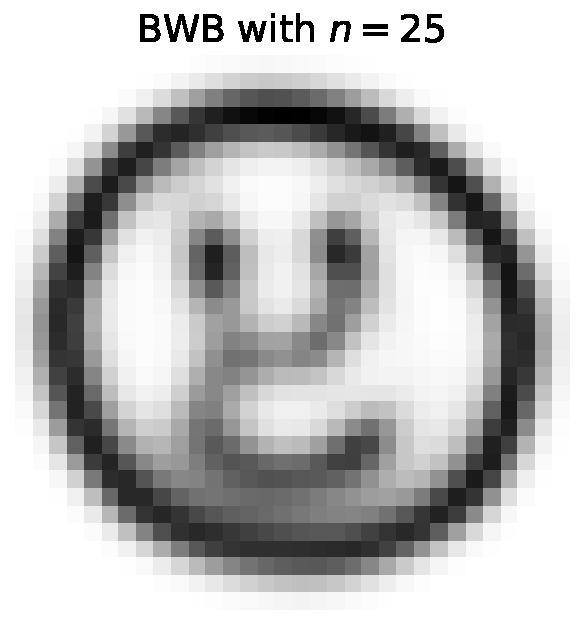
\includegraphics[height=6cm]{img/bwb/BWB-n-data-25.pdf}
        \caption{Baricentro con $n=25$.}
        \label{fig:bwb-n-data-25}
    \end{subfigure}
    \caption{Resultados de los experimentos para el cálculo del BWB con $n=25$.}
    \label{fig:bwb-experiments-n-25}
\end{figure}

% n = 50
\begin{figure}[H]
    \begin{subfigure}[t]{0.49\textwidth}
        \centering
        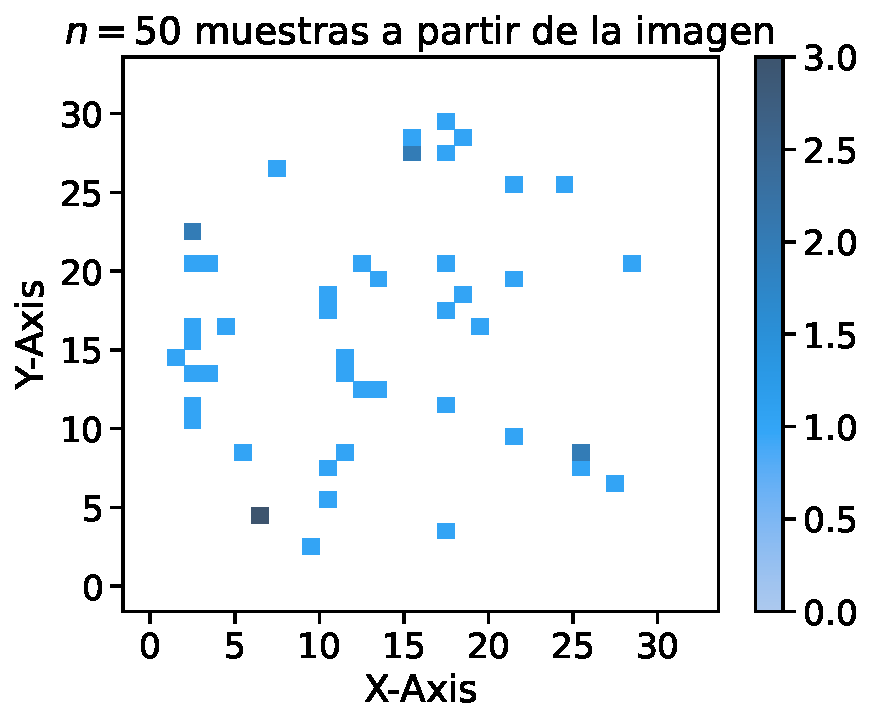
\includegraphics[height=6cm]{img/bwb/samples-hist-n-50.pdf}
        \caption{Histograma de los datos con $n=50$.}
        \label{fig:samples-hist-n-50}
    \end{subfigure}
    \hfill
    \begin{subfigure}[t]{0.49\textwidth}
        \centering
        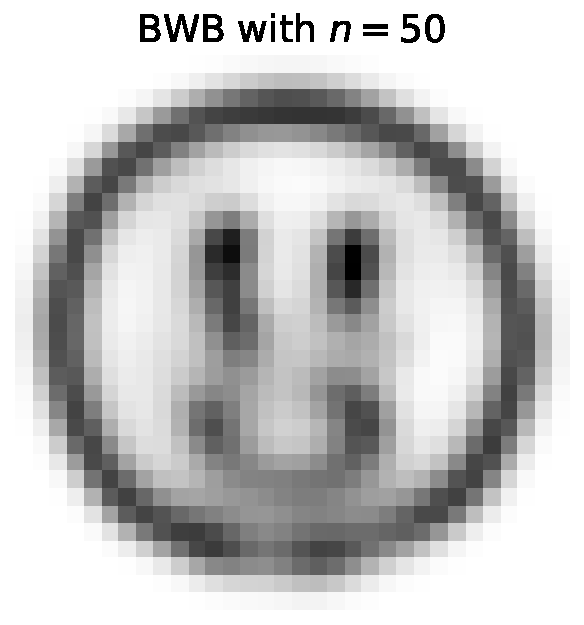
\includegraphics[height=6cm]{img/bwb/BWB-n-data-50.pdf}
        \caption{Baricentro con $n=50$.}
        \label{fig:bwb-n-data-50}
    \end{subfigure}
    \caption{Resultados de los experimentos para el cálculo del BWB con $n=50$.}
    \label{fig:bwb-experiments-n-50}
\end{figure}

A partir de las figuras anteriores se puede observar que a medida que se aumenta el número de datos $n$, el baricentro de Wasserstein Bayesiano se parece más al modelo original $\tilde\mu$, pero de manera difuminada, como lo son los baricentros clásicos (Fig.~\ref{fig:barycenters}). Esto es lo esperable, pues a medida que se aumenta el número de datos, la posterior se concentra más en el modelo original, lo que se traduce en un baricentro más parecido a $\tilde\mu$.


\subsection{Conclusiones}\label{ssec:bwb-conclusiones}  % MARK: - Conclusiones

\RED[inline]{Revisar esta conclusión}
En vista a los resultados obtenidos, se concluye que el enfoque de obtener muestreos a partir de la posterior usando una red generativa como prior ha resultado de manera satisfactoria. Además, que la implementación del BWB ha resultado exitoso y que se ha logrado obtener baricentros de manera efectiva.
